%%
% S20 CSCI 470 Web Science
%
% Battleship Protocol
%
% Phillip J. Curtiss, PhD, Associate Professor
% pcurtiss@mtech.edu, 406-496-4807
% Department of Computer Science, Montana Tech
%%
\documentclass[10pt]{article}
\usepackage[T1]{fontenc}
\usepackage[margin=1in,headheight=20pt]{geometry}
\usepackage{fancyhdr}
\usepackage{graphicx}
\usepackage[sc]{titlesec}
\usepackage{lastpage}
\usepackage{tikz}
\usetikzlibrary{calc,shapes,positioning,arrows}
\usepackage{listings}
\usepackage{textcomp}

%%
% S18 CSCI470 - Web Science
% Exam-1 
%
% Languages Defined for the lstlisting package
% Languages include: css, html5, JavaScript
%
% Phillip J. Curtiss, Assistant Professor, 
% Department of Computer Science, Montana Tech
% pcurtiss@mtech.edu, 406-496-4807
% (c) 2018 All Rights Reserved
% cspell:ignore bootloader eqexam tabsize setspace
%%
% Color Specifications for code decorations
\definecolor{lightgray}{rgb}{0.95, 0.95, 0.95}
\definecolor{darkgray}{rgb}{0.4, 0.4, 0.4}
\definecolor{purple}{rgb}{0.65, 0.12, 0.82}
\definecolor{editorGray}{rgb}{0.95, 0.95, 0.95}
\definecolor{editorOcher}{rgb}{1, 0.5, 0} % #FF7F00 -> rgb(239, 169, 0)
\definecolor{editorGreen}{rgb}{0, 0.5, 0} % #007C00 -> rgb(0, 124, 0)
%%
% Custom lstlisting Language for HTML5
\lstdefinelanguage{HTML5}{
  language=html,
  sensitive=true,	
  alsoletter={<>=-},	
  morecomment=[s]{<!-}{-->},
  tag=[s],
  otherkeywords={
  % General
  >,
  % Standard tags
	<!DOCTYPE,
  </html, <html, <head, <title, </title, <style, </style, <link, </head, <meta, />,
	% body
	</body, <body,
	% Divs
	</div, <div, </div>, 
	% Paragraphs
	</p, <p, </p>,
	% scripts
	</script, <script,
  % More tags...
  <canvas, /canvas>, <svg, <rect, <animateTransform, </rect>, </svg>, <video, <source, <iframe, </iframe>, </video>, <image, </image>
  },
  ndkeywords={
  % General
  =,
  % HTML attributes
  charset=, src=, id=, width=, height=, style=, type=, rel=, href=,
  % SVG attributes
  fill=, attributeName=, begin=, dur=, from=, to=, poster=, controls=, x=, y=, repeatCount=, xlink:href=,
  % CSS properties
  margin:, padding:, background-image:, border:, top:, left:, position:, width:, height:,
	% CSS3 properties
  transform:, -moz-transform:, -webkit-transform:,
  animation:, -webkit-animation:,
  transition:,  transition-duration:, transition-property:, transition-timing-function:,
  }
}
%%
% Custom lstlisting Language for JavaScript
\lstdefinelanguage{JavaScript}{
  morekeywords={typeof, new, true, false, catch, function, return, null, catch, switch, var, if, in, while, do, else, case, break},
  morecomment=[s]{/*}{*/},
  morecomment=[l]//,
  morestring=[b]",
  morestring=[b]'
}
%%
% Custom lstlisting Language for CSS
\lstdefinelanguage{CSS}{
  keywords={color,background-image:,margin,padding,font,weight,display,position,top,left,right,bottom,list,style,border,size,white,space,min,width, transition:, transform:, transition-property, transition-duration, transition-timing-function},	
  sensitive=true,
  morecomment=[l]{//},
  morecomment=[s]{/*}{*/}, 
  morestring=[b]',
  morestring=[b]",
  alsoletter={:},
  alsodigit={-}
}


\lstloadlanguages{HTML5,JavaScript,CSS}
\lstset{
   numbers=left,
   upquote=true,
   breaklines=true,
	backgroundcolor=\color{black!7},
	tabsize=2,
	language=JavaScript
}

\makeatletter
   \tikzset{reset preactions/.code={\def\tikz@preactions{}}}
\makeatother

%% 
% First Page Style
\fancypagestyle{project}{%
   \fancyhf{}% Clear all settings
   \lhead{%
      {\bfseries{} Battleship Game Protocol} \\
      {S20 CSCI470 Web Science} \\
      {Reference: Node, HTTP, SSE}}
   \rhead{Assigned: 2019-03-23 \\
          Due Date: 2019-04-06}
   \lfoot{Phillip J. Curtiss, Associate Professor \textbullet\ 
          Department of Computer Science \textbullet\ Montana Tech}
   \rfoot{Page~\thepage~of~\pageref{LastPage}}
   \renewcommand{\headrulewidth}{0.4pt}
   \renewcommand{\footrulewidth}{0.4pt}
}

\begin{document}
\pagestyle{project}

\section*{Summary:}

\begin{center}
   \renewcommand{\arraystretch}{1.2}
   \begin{tabular}{r p{4.5in}}
      \hline 
      Abstract: & Battleship Game Protocol \\
      Objectives: & \begin{enumerate}
                     \item Node Route Class 
                     \item Node Modules - Export and Import
                     \item Application Protocol 
                     \item REST Design, End-Points, Methods
                     \item SSE, JSON
                     \item HTTP Client in Node Server
                    \end{enumerate} \\
      Grading: & 45 pts - \\[-3 em]
               & \begin{tabbing}
                  C+ \= $\ge$ 34.65; C+ \= $\ge$ 32.85; C+ \= $\ge$ 31.75; D+ \= $\ge$ 30.15; D+ \= $\ge$ 28.35; D+ \= $\ge$ 27 \kill
               ~ \> \hspace{3.7em}    A \> $\ge$ 41.85; A- \> $\ge$ 40.50; B+ \> $\ge$ 39.15; B \> $\ge$ 37.35; B- \> $\ge$ 36; \\
                C+ \> $\ge$ 34.65; C \> $\ge$ 32.85; C- \> $\ge$ 31.75; D+ \> $\ge$ 30.15; D \> $\ge$ 28.35; D- \> $\ge$ 27 
               \end{tabbing} \\
      Outcomes: & R2 (CAC-a,c,i, j, k; EAC-a, b, c, e, k, 1, 2); R5 (CAC-a, i; EAC-a, k)  \\
                & (see syllabus for description of course outcomes) \\ \hline
   \end{tabular}
\end{center}

\section*{Project Description:}

\begin{center}
   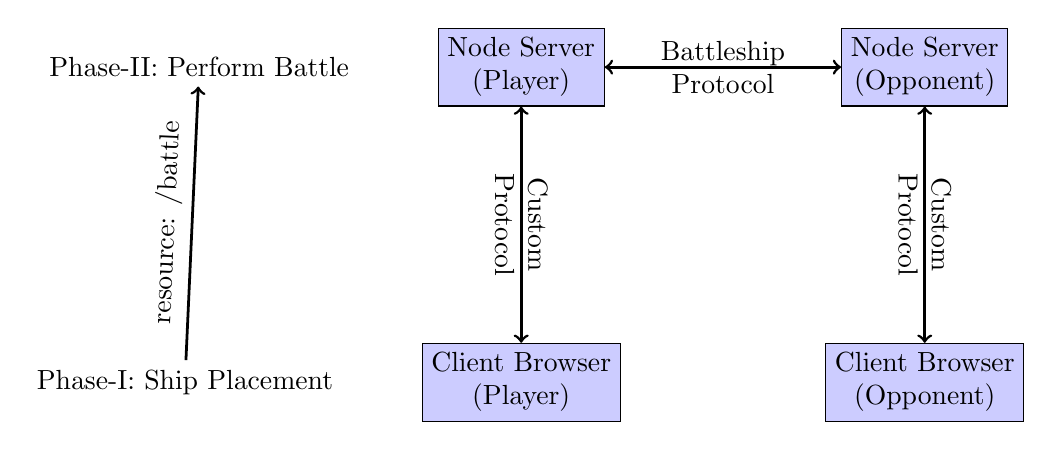
\begin{tikzpicture}[
      clear/.style={draw=none,fill=none,align=center},
      every node/.style={draw, rectangle, fill=blue!20, align=center},
      every edge/.style={draw, <->, line width=1.0pt}
   ]
      \node (N1) {Node Server\\(Player)};
      \node[right=3cm of N1] (N2) {Node Server\\(Opponent)};
      \node[below=3cm of N1] (C1) {Client Browser\\(Player)};
      \node[below=3cm of N2] (C2) {Client Browser\\(Opponent)};

      \path (N1) edge node[clear,sloped] {Custom\\Protocol} (C1);
      \path (N2) edge node[clear,sloped] {Custom\\Protocol} (C2);
      \path (N1) edge node[clear] {Battleship\\Protocol}  (N2);

      \node[clear,left=of N1] (PII) {Phase-II: Perform Battle};
      \node[clear,left=of C1] (PI) {Phase-I: Ship Placement};
      \begin{scope}[every edge/.style={draw,->,line width=1.0pt}]
         \path (PI) edge node[clear,above,sloped] {resource: /battle} (PII);
      \end{scope}
   \end{tikzpicture}
\end{center}

During Phase-I of the game, the end-user uses the client browser to either (a) place their ships on their ocean grid, or (b) load a pre-configured ocean grid from their node server. Once their ships have been placed, the user initiates a battle request by performing a request to the \verb|/battle| resource (see below for details). This should disallow any changes to the player's ocean grid and initiate Phase-II of the game, performing battle with an opponent. 

During the Phase-II of the game, the user initiating the session request will be known as the \emph{player} and the user fulfilling the session request with a response will be known as the \emph{opponent}. The process of battle follows the sequence of \emph{request} and \emph{response} pairs between the player's node server and the opponent's node server. 

Create a new route class to implement the Battleship game protocol. The game protocol must be implemented exactly according to the specification provided herein or the ability to participate in a game with another player will not work as expected. The route class will need to import a reference to a function exported from the SSE module that will allow code within the protocol module to send messages to the front-end client game board application via the HTML5 Server Sent Events API. 

Also, implement a tile selection strategy used when firing on your opponents ships. This strategy can be as sophisticated as you like, or completely random. The starter files for this project already implement a completely random tile selection strategy. A reasonable strategy should operate in two phases - the first when no opponent ship is presently hit, and the second when an opponent ship has been hit. Be careful with this component of your project as the tile selection strategy should not take a large amount of processing time given the single-threaded nature of the Node server. 

\subsection*{Battleship Game Protocol:}

\begin{quote}
   \begin{description}
      \item[Resource End-Point:] \lstinline|[GET]/battle/:filename[/:url]| Change to the battle mode and optionally engage with opponent at \verb|url|. Load the game state from the file given in \verb|filename|. If the \verb|url| is not specified, load the game state and then wait for an opponent to request a session (see \verb|/session| endpoint below).
      
      \item[Request Body:] \emph{There is no request body.}
      
      \item[Status Codes:] ~
         \begin{description}
            \item[200 OK -] Entered Battle Mode (see response message)
            \item[400 Bad Request -] Server could not understand the request
            \item[401 Unauthorized -] Not an authorized client of the node server
            \item[404 Not Found -] Game state filename could not be found on the server  
         \end{description} 

      \item[Response Body if Status Code 200:]
         \begin{lstlisting}[gobble=12]
            {
               // game model - bsState JSON 
            }
         \end{lstlisting}

         \paragraph{Postcondition:} Server is in phase-II, battle mode.

      \item[Response Body if Status Code 400:]
         \begin{lstlisting}[gobble=12]
            {
               'request': // full request provided
            }
         \end{lstlisting}

         \paragraph{Postcondition:} Server remains in phase-I.

      \item[Response Body if Status Code 401:]
         \begin{lstlisting}[gobble=12]
            {
               'links': {
                  'auth': {
                     'href': 'https//csdept16.mtech.edu:XXXXX/auth',
                     'rel': '/auth'
                  }
               }
            } // XXXXX - port assigned to each student node instance
         \end{lstlisting}

         \paragraph{Postcondition:} Server remains in phase-I.

      \item[Response Body if Status Code 404:]
         \begin{lstlisting}[gobble=12]
            {
               'filename': // filename provided in request
            }
         \end{lstlisting}

         \paragraph{Postcondition:} Server remains in phase-I.

      \newpage 
      \item[Resource End-Point:] \lstinline|[POST]/session| Request to engage in a battle session with an opponent identified in the \verb|url| of the \verb|battle| request. 
      
      \item[Request Body:]
         \begin{lstlisting}[gobble=12]
            {
               'opponentURL': // your url with port,
               ['latency': 5000] // optional latency between 2000 - 10000 ms
            }
         \end{lstlisting}
      
      \item[Status Codes:] ~
         \begin{description}
            \item[200 OK -] If the opponent creates a session with the player (requester)
            \item[400 Bad Request -] Server could not understand the request
            \item[403 Forbidden -] Opponent is already in another session
            \item[412 Precondition Failed -] Opponent is not in \emph{battle} phase   
         \end{description}

      \item[Response Body if Status Code 200:]
         \begin{lstlisting}[gobble=12]
            {
               'session': // session identifier ,
               'roll': // 1 or 0,
               'names': // [<system name text>, <player name text>],
               'epoc': // unix time stamp (in ms since 1/1/1970 00:00:00),
               'latency': 5000 // value between 2000 - 10000 (in ms)
            }
         \end{lstlisting}
         \begin{itemize}
            \item \lstinline|Roll = Math.floor(Math.random()*2);|
            
                  Player's turn when \lstinline|roll == 0|; \\
                  Opponent's turn when \lstinline|roll == 1|.
            \item \lstinline|epoc = (new Date()).getTime();| 
            
                  Number of milliseconds since Unix EPIC (1/1/1970 00:00:00)

            \item System name is the text name of the system providing the response.
            
                  Must be between 3 and 20 characters.
            \item Player name is the text name of the user of the system.
            
                  Must be between 3 amd 20 characters.

            \item The session-id is comprised of:
               \begin{itemize}
                  \item \lstinline|md5(localIPAddr + removeIPAddr + epoc);|
                  \item \lstinline|localIPAddr| is the IP address of the node server forming the response
                  \item \lstinline|removeIPAddr| is the IP address of the node server of the requester
                  \item \lstinline|epoc| is as previously computed
                  \item MD5 is the message digest hash of the concatenated strings as shown
               \end{itemize}

            \item Latency request:
               \begin{itemize}
                  \item Is just a request,
                  \item must be between 2000 and 10000 ms (2s and 10s respectively)
                  \item Is completely optional for honoring the request
                  \item default should remain 5000 ms
               \end{itemize}
         \end{itemize}

         \paragraph{Postcondition:} Battle session established; servers take turns issuing \verb|/target| endpoint requests until the game is completed.
      
      \item[Response Body if Status Code 400:]
         \begin{lstlisting}[gobble=12]
            {
               'request': // full request provided
            }
         \end{lstlisting}

         \paragraph{Postcondition:} Server remains in battle mode; session with opponent is not established; error should be reported to client front-end.

      \item[Response Body if Status Code 403:]
         \begin{lstlisting}[gobble=12]
            {
               'opponent': ['system name', 'player name']
            }
         \end{lstlisting}

         \paragraph{Postcondition:} Server remains in battle mode; session with opponent is not established; error should be reported to client front-end.

      \item[Response Body if Status Code 412:] \emph{There is no response body.}
      
         \paragraph{Postcondition:} Server remains in phase-I.
      
      \item[Resource End-Point:] \lstinline|[DELETE]/session/<session-id| Request to terminate existing session with an opponent and reset game state
      \item[Request Body:] \emph{There is no request body.}
      \item[Status Codes:] ~
         \begin{description}
            \item[200 OK -] If the opponent terminates the session
            \item[400 Bad Request -] Server could not understand the request
            \item[403 Forbidden -] No access rights to delete session-id
            \item[404 Not Found -] Provided session-id is not valid 
            \item[412 Precondition Failed -] Opponent is not in \emph{battle} phase    
         \end{description}

      \item[Response Body if Status Code is 200:]
         \begin{lstlisting}[gobble=12]
            {
               'session': 'session-id',
               'duration': // total time spent in session (in ms)
            }
         \end{lstlisting}

         \paragraph{Postcondition:} Session is destroyed; server leaves phase-II; server enters phase-I.

      \item[Response Body if Status Code is 400:]
         \begin{lstlisting}[gobble=12]
            {
               'request': // full request provided
            }
         \end{lstlisting}

         \paragraph{Postcondition:} Session remains intact.

      \item[Response Body if Status Code is 403:]
         \begin{lstlisting}[gobble=12]
            {
               'session': 'session-id'
            }
         \end{lstlisting}

         \paragraph{Postcondition:} Session remains intact.

      \item[Response Body if Status Code is 404:]
         \begin{lstlisting}[gobble=12]
            {
               'session': 'session-id'
            }
         \end{lstlisting}

         \paragraph{Postcondition:} Session remains intact.

      \item[Response Body if Status Code is 412:] \emph{There is no response body.}
      
         \paragraph{Postcondition:} Server remains in phase-I.
      
      \item[Resource End-Point:] \lstinline|[POST]/target| Fire onto your opponent's target grid at a given tile location.
      \item[Request Body:]
         \begin{lstlisting}[gobble=12]
            {
               'session': 'session-id',
               'tile': // tile specification
            }
         \end{lstlisting}
         \begin{itemize}
            \item \lstinline|tile == [A..J][0..9]|, in \emph{row}, \emph{column} format.
         \end{itemize}
      \item[Status Codes:] ~
         \begin{description}
            \item[200 OK -] Opponent accepts the target request
            \item[400 Bad Request -] Server could not understand the request
            \item[401 Unauthorized -] Not a valid session-id
            \item[403 Forbiddien -] Not the opponent's turn 
            \item[412 Precondition Failed -] Opponent is not in \emph{battle} phase    
         \end{description}

      \item[Response Body if Status Code is 200:]
         \begin{lstlisting}[gobble=12]
            {
               'status': 'MISS' | 'CARRIER' | 'BATTLESHIP' | 
                         'CRUISER' | 'SUBMARINE' | 'DESTROYER',
               'tile': 'RC',
               'disposition': 'INPROGRESS' | 'WIN'
            }
         \end{lstlisting}

         \paragraph{Postcondition:} After processing response, appropriate SSE message should be sent to the front-end indicating disposition of the target attempt; turn should be updated.

      \item[Response Body if Status Code is 400:]
         \begin{lstlisting}[gobble=12]
            {
               'request': // full request provided
            }
         \end{lstlisting}

         \paragraph{Postconditin:} Turn should not be updated.

      \item[Response Body if Status Code is 401:] \emph{There is no response body.}
      
         \paragraph{Postcondition:} Turn should not be updated.

      \item[Response Body if status Code is 403:] \emph{There is no response body.}
      
         \paragraph{Postcondition:} Turn should not be updated.
      
      \item[Response Body if Status Code is 412:] \emph{There is no response body.} 
    
         \paragraph{Postcondition:} Turn should not be updated.
   \end{description}
\end{quote}

\newpage
\subsection*{Obtaining Project Files:}

   \begin{enumerate}
      \item Logon to \verb|gitlab.cs.mtech.edu| and locate the project \verb|bsBattleProtocol| under the \verb|S20 CSCI470| (sub)group, and then fork this project into your own account.
      \item Navigate to your own account and locate the \verb|bsBattleProtocol| project  just forked, and copy the project url
      \item Next, logon to \verb|csdept16.mtech.edu| using your Department username and password. 
      \item Execute the \verb|mkdir ~/CSCI470/Projects/| command, which will create a projects folder if not already created.
      \item Execute the \verb|cd ~/CSCI470/Projects| command, which will change the current working directory to the specified parameter. 
      \item Issue the command \verb|git clone <project_url>|, where \verb|<project_url>| is the url you copied in the above step. This will create the project folder inside your \verb|~/CSCI470/Projects| directory,
      \item Execute the command \verb|cd bsBattleProtocol| to enter the project directory.
      \item Continue with the specific project activities below.
   \end{enumerate}

\section*{Project Activities:}

Please perform the following activities in the completion of the lab assignment.

\begin{enumerate}
	\item After cloning the project, navigate to its folder and incorporate your previous project files (route classes and and changes in \verb|app.js|) with this project. 
   
   \item Change to the \verb|routes| directory and review the code and comments in the \verb|bsProtocol.js| file. 
   
   \item Implement the resource end-points in the file to conform to the REST protocol as documented herein. 
   
   \item Review the code and comments in the \verb|bsStrategy.js| file. This is an implementation of a completely random tile selection strategy. You should feel free to use this strategy or update this strategy with an alternative. 
   
   \item Modify the \emph{server sent events} route class from the previous project such that the \emph{protocol} module (this module) can send events to its client to update either the \emph{ocean grid} or the \emph{target grid}. This likely will require an update to the exported function from the \emph{sse} module as well. 
   
   \item On your game board (client) implement the following:
   \begin{enumerate}
      \item Attach a listener to the \emph{New Game} menu item that:
      \begin{enumerate}
         \item Will prompt the user for:
         \begin{enumerate}
            \item the name (filename) of a previously saved game state 
            \item (optionally) a url of an opponent, including any port
            \item (optionally) a latency between 2000 and 5000
         \end{enumerate}

         \item will form a request to the client's \verb|/battle| resource end-point.
         
         \item will disallow the placement or movement of any ships on the game board
         
         \item disable the load and save game menu items
      \end{enumerate}
   
      \item Attached a listener to the \emph{Exit} menu item that:
      \begin{enumerate}
         \item will request from the use to confirm termination of the current game
         
         \item if the user terminates a current game, reset the game board
         
         \item terminate the SSE - via closing the \verb|EventSource| object
      \end{enumerate}
      
      \item If the SSE messages a \verb|WIN|, indicate to the user and reset the game board.
   \end{enumerate}
\end{enumerate}

\newpage
\section*{Project Grading:}

The project must compile without errors (ideally without warnings) and should not fault upon execution. All errors should be caught if thrown and handled in a rational manner. Grading will follow the \emph{project grading rubric} shown in figure~\ref{fig:grading}.

\begin{figure}
 \caption{Programming Project Grading Rubric} \label{fig:grading}
 \begin{center}
   \renewcommand{\arraystretch}{1.5}
   \footnotesize
   \begin{tabular}{c p{1.2in} p{1.2in} p{1.2in} p{1.2in}} 
      Attribute (pts) & \multicolumn{1}{c}{Exceptional (1)} & \multicolumn{1}{c}{Acceptable (0.8)} & \multicolumn{1}{c}{Amateur (0.7)} & \multicolumn{1}{c}{Unsatisfactory (0.6)} \\ \hline
      Specification (10) & The program works and meets all of the specifications.
                         & The program works and produces correct results and displays them correctly. It also meets most of the other specifications.
                         & The program produces correct results, but does not display them correctly.
                         & The program produces incorrect results. \\
      Readability (10) & The code is exceptionally well organized and very easy to follow.
                       & The code is fairly easy to read.
                       & The code is readable only by someone who knows what it is supposed to be doing.
                       & The code is poorly organized and very difficult to read. \\
      Reusability (10) & The code could be reused as a whole or each routine could be reused.
                       & Most of the code could be reused in other programs. 
                       & Some parts of the code could be reused in other programs. 
                       & The code is not organized for reusability. \\
      Documentation (10) & The documentation is well written and clearly explains what the code is                        accomplishing and how.
                         & The documentation consists of embedded comments and some simple header documentation that is somewhat useful in understanding the code. 
                         & The documentation is simply comments embedded in the code with some simple header comments separating routines. 
                         & The documentation is simply comments embedded in the code and does not help the reader understand the code. \\
      Efficiency (5) & The code is extremely efficient without sacrificing readability and                            understanding.
                     & The code is fairly efficient without sacrificing readability and understanding. 
                     & The code is brute force and unnecessarily long.
                     & The code is huge and appears to be patched together. \\
      Delivery (total) & The program was delivered on-time.
                       & The program was delivered within a week of the due date. 
                       & The program was delivered within 2-weeks of the due date. 
                       & The code was more than 2-weeks overdue. \\ \hline
      \multicolumn{5}{p{\textwidth}}{The \emph{delivery} attribute weights will be applied to the total score from the other attributes. That is, if a project scored 36 points total for the sum of \emph{specification}, \emph{readability}, \emph{reusability}, \emph{documentation} and \emph{efficiency} attributes, but was turned in within 2-weeks of the due date, the project score would be $36 \cdot 0.7 = 25.2$.}
   \end{tabular}
 \end{center}
\end{figure}

\section*{Collaboration Opportunities:}

You may collaborate with up to one other person on this project - but you must cite, in the code (html, css, js) each students' contribution.

\end{document}